\documentclass{standalone}
\usepackage{tikz}
\usetikzlibrary{patterns, positioning}
\usepackage[sfdefault]{ClearSans} %% option 'sfdefault' activates Clear Sans as the default text font
\usepackage[T1]{fontenc}

\begin{document}
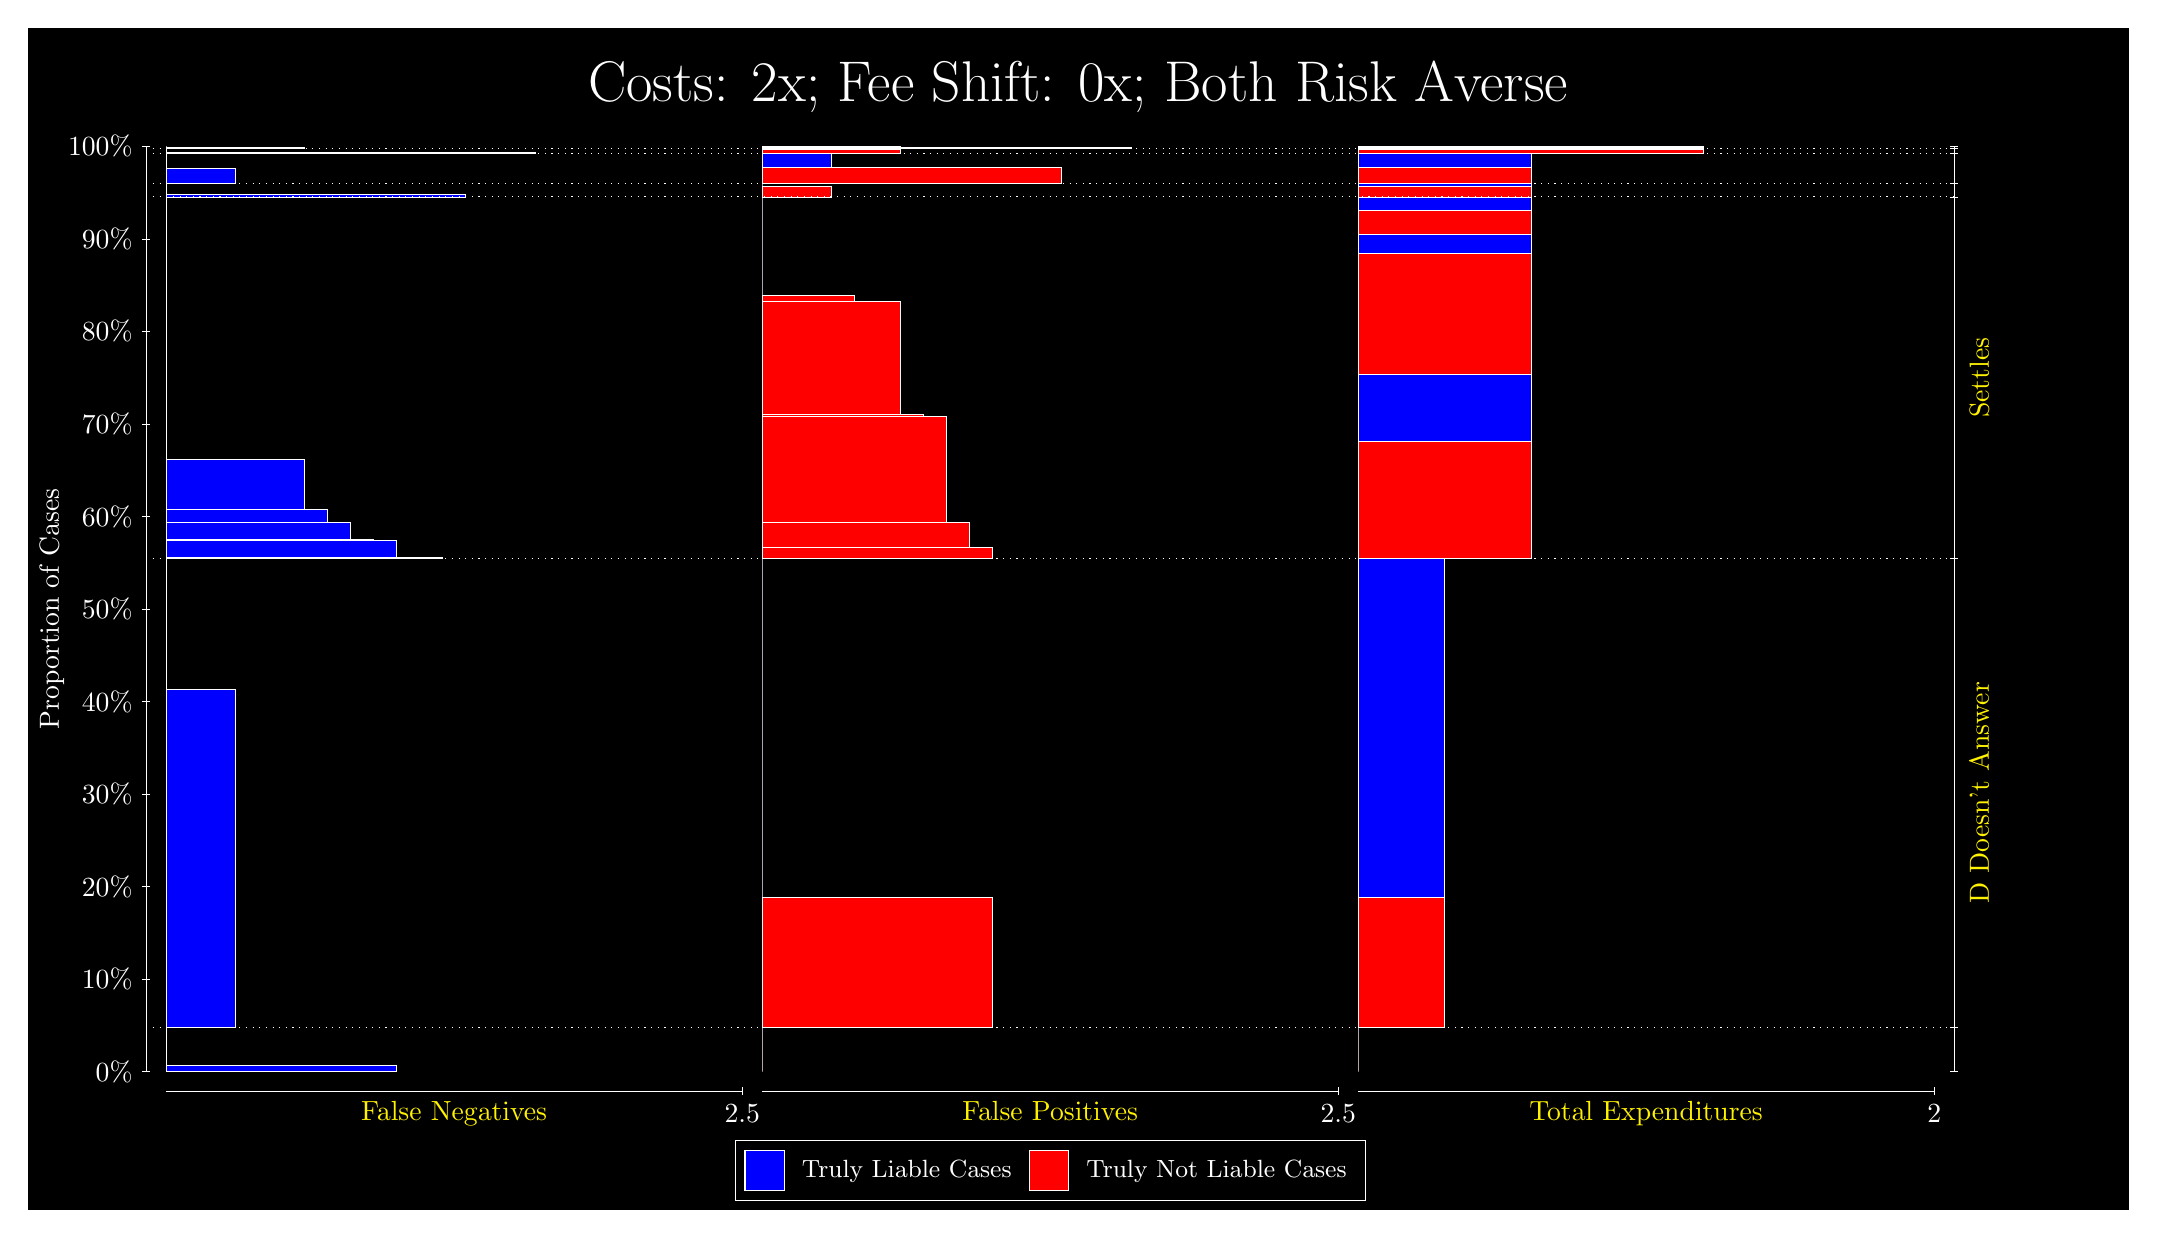
\begin{tikzpicture}
\draw[fill=black] (0,0) rectangle (26.667,15);
\draw[text=white] (0,13.5) rectangle (26.667,15) node[midway] {\huge Costs: 2x; Fee Shift: 0x; Both Risk Averse};
\draw[white, very thin] (1.5,1.75) -- (1.5,13.5);
\node[rotate=90, text=white, anchor=center] at (0.3, 7.625) {Proportion of Cases};
\draw[white, very thin] (1.45,1.75) -- (1.55,1.75);
\node[text=white, anchor=east] at (1.45, 1.75) {0\%};
\draw[white, very thin] (1.45,2.925) -- (1.55,2.925);
\node[text=white, anchor=east] at (1.45, 2.925) {10\%};
\draw[white, very thin] (1.45,4.1) -- (1.55,4.1);
\node[text=white, anchor=east] at (1.45, 4.1) {20\%};
\draw[white, very thin] (1.45,5.275) -- (1.55,5.275);
\node[text=white, anchor=east] at (1.45, 5.275) {30\%};
\draw[white, very thin] (1.45,6.45) -- (1.55,6.45);
\node[text=white, anchor=east] at (1.45, 6.45) {40\%};
\draw[white, very thin] (1.45,7.625) -- (1.55,7.625);
\node[text=white, anchor=east] at (1.45, 7.625) {50\%};
\draw[white, very thin] (1.45,8.8) -- (1.55,8.8);
\node[text=white, anchor=east] at (1.45, 8.8) {60\%};
\draw[white, very thin] (1.45,9.975) -- (1.55,9.975);
\node[text=white, anchor=east] at (1.45, 9.975) {70\%};
\draw[white, very thin] (1.45,11.15) -- (1.55,11.15);
\node[text=white, anchor=east] at (1.45, 11.15) {80\%};
\draw[white, very thin] (1.45,12.325) -- (1.55,12.325);
\node[text=white, anchor=east] at (1.45, 12.325) {90\%};
\draw[white, very thin] (1.45,13.5) -- (1.55,13.5);
\node[text=white, anchor=east] at (1.45, 13.5) {100\%};

\draw[white, very thin] (24.457,1.75) -- (24.457,13.5);
\draw[white, very thin] (24.407,1.75) -- (24.507,1.75);
\node[anchor=west] at (24.407, 1.75) {};
\draw[white, very thin] (24.407,2.312) -- (24.507,2.312);
\node[anchor=west] at (24.407, 2.312) {};
\draw[white, very thin] (24.407,8.2644) -- (24.507,8.2644);
\node[anchor=west] at (24.407, 8.2644) {};
\draw[white, very thin] (24.407,12.858) -- (24.507,12.858);
\node[anchor=west] at (24.407, 12.858) {};
\draw[white, very thin] (24.407,13.033) -- (24.507,13.033);
\node[anchor=west] at (24.407, 13.033) {};
\draw[white, very thin] (24.407,13.409) -- (24.507,13.409);
\node[anchor=west] at (24.407, 13.409) {};
\draw[white, very thin] (24.407,13.471) -- (24.507,13.471);
\node[anchor=west] at (24.407, 13.471) {};
\draw[white, very thin] (24.407,13.5) -- (24.507,13.5);
\node[anchor=west] at (24.407, 13.5) {};

\draw[white, very thin, fill=blue] (1.75,1.75) rectangle (4.6775,1.8248);
\draw[white, very thin, fill=red] (1.75,1.8248) rectangle (1.75,2.312);
\draw[white, very thin, fill=blue] (1.75,2.312) rectangle (2.6283,6.6096);
\draw[white, very thin, fill=red] (1.75,6.6096) rectangle (1.75,8.2644);
\draw[white, very thin, fill=blue] (1.75,8.2644) rectangle (5.2631,8.276);
\draw[white, very thin, fill=blue] (1.75,8.276) rectangle (4.6775,8.4997);
\draw[white, very thin, fill=blue] (1.75,8.4997) rectangle (4.3848,8.5075);
\draw[white, very thin, fill=blue] (1.75,8.5075) rectangle (4.092,8.7202);
\draw[white, very thin, fill=blue] (1.75,8.7202) rectangle (3.7993,8.885);
\draw[white, very thin, fill=blue] (1.75,8.885) rectangle (3.5065,9.5202);
\draw[white, very thin, fill=red] (1.75,9.5202) rectangle (1.75,12.858);
\draw[white, very thin, fill=blue] (1.75,12.858) rectangle (5.5558,12.894);
\draw[white, very thin, fill=red] (1.75,12.894) rectangle (1.75,13.033);
\draw[white, very thin, fill=blue] (1.75,13.033) rectangle (2.6283,13.215);
\draw[white, very thin, fill=red] (1.75,13.215) rectangle (1.75,13.409);
\draw[white, very thin, fill=blue] (1.75,13.409) rectangle (6.4341,13.423);
\draw[white, very thin, fill=red] (1.75,13.423) rectangle (1.75,13.471);
\draw[white, very thin, fill=blue] (1.75,13.471) rectangle (3.5065,13.486);
\draw[white, very thin, fill=red] (1.75,13.486) rectangle (1.75,13.5);
\draw[white, very thin, fill=red] (9.3189,1.75) rectangle (9.3189,2.2372);
\draw[white, very thin, fill=blue] (9.3189,2.2372) rectangle (9.3189,2.312);
\draw[white, very thin, fill=red] (9.3189,2.312) rectangle (12.246,3.9668);
\draw[white, very thin, fill=blue] (9.3189,3.9668) rectangle (9.3189,8.2644);
\draw[white, very thin, fill=red] (9.3189,8.2644) rectangle (12.246,8.4142);
\draw[white, very thin, fill=red] (9.3189,8.4142) rectangle (11.954,8.7196);
\draw[white, very thin, fill=red] (9.3189,8.7196) rectangle (11.661,10.066);
\draw[white, very thin, fill=red] (9.3189,10.066) rectangle (11.368,10.094);
\draw[white, very thin, fill=red] (9.3189,10.094) rectangle (11.075,11.53);
\draw[white, very thin, fill=red] (9.3189,11.53) rectangle (10.49,11.602);
\draw[white, very thin, fill=blue] (9.3189,11.602) rectangle (9.3189,12.858);
\draw[white, very thin, fill=red] (9.3189,12.858) rectangle (10.197,12.998);
\draw[white, very thin, fill=blue] (9.3189,12.998) rectangle (9.3189,13.033);
\draw[white, very thin, fill=red] (9.3189,13.033) rectangle (13.125,13.228);
\draw[white, very thin, fill=blue] (9.3189,13.228) rectangle (10.197,13.409);
\draw[white, very thin, fill=red] (9.3189,13.409) rectangle (11.075,13.457);
\draw[white, very thin, fill=blue] (9.3189,13.457) rectangle (9.3189,13.471);
\draw[white, very thin, fill=red] (9.3189,13.471) rectangle (14.003,13.484);
\draw[white, very thin, fill=blue] (9.3189,13.484) rectangle (11.075,13.5);
\draw[white, very thin, fill=red] (16.888,1.75) rectangle (16.888,2.2372);
\draw[white, very thin, fill=blue] (16.888,2.2372) rectangle (16.888,2.312);
\draw[white, very thin, fill=red] (16.888,2.312) rectangle (17.986,3.9668);
\draw[white, very thin, fill=blue] (16.888,3.9668) rectangle (17.986,8.2644);
\draw[white, very thin, fill=red] (16.888,8.2644) rectangle (19.083,9.7602);
\draw[white, very thin, fill=blue] (16.888,9.7602) rectangle (19.083,10.608);
\draw[white, very thin, fill=red] (16.888,10.608) rectangle (19.083,12.145);
\draw[white, very thin, fill=blue] (16.888,12.145) rectangle (19.083,12.388);
\draw[white, very thin, fill=red] (16.888,12.388) rectangle (19.083,12.693);
\draw[white, very thin, fill=blue] (16.888,12.693) rectangle (19.083,12.858);
\draw[white, very thin, fill=red] (16.888,12.858) rectangle (19.083,12.998);
\draw[white, very thin, fill=blue] (16.888,12.998) rectangle (19.083,13.033);
\draw[white, very thin, fill=red] (16.888,13.033) rectangle (19.083,13.228);
\draw[white, very thin, fill=blue] (16.888,13.228) rectangle (19.083,13.409);
\draw[white, very thin, fill=red] (16.888,13.409) rectangle (21.279,13.457);
\draw[white, very thin, fill=blue] (16.888,13.457) rectangle (21.279,13.471);
\draw[white, very thin, fill=red] (16.888,13.471) rectangle (21.279,13.484);
\draw[white, very thin, fill=blue] (16.888,13.484) rectangle (21.279,13.5);
\draw[white, dotted] (1.5,2.312) -- (24.457,2.312);
\draw[white, dotted] (1.5,8.2644) -- (24.457,8.2644);
\draw[white, dotted] (1.5,12.858) -- (24.457,12.858);
\draw[white, dotted] (1.5,13.033) -- (24.457,13.033);
\draw[white, dotted] (1.5,13.409) -- (24.457,13.409);
\draw[white, dotted] (1.5,13.471) -- (24.457,13.471);
\draw[white, very thin] (1.75,1.5) -- (9.0689,1.5);
\node[text=yellow, anchor=north] at (5.4094, 1.5) {False Negatives};
\draw[white, very thin] (9.0689,1.45) -- (9.0689,1.55);
\node[text=white, anchor=north] at (9.0689, 1.45) {2.5};

\draw[white, very thin] (9.3189,1.5) -- (16.638,1.5);
\node[text=yellow, anchor=north] at (12.978, 1.5) {False Positives};
\draw[white, very thin] (16.638,1.45) -- (16.638,1.55);
\node[text=white, anchor=north] at (16.638, 1.45) {2.5};

\draw[white, very thin] (16.888,1.5) -- (24.207,1.5);
\node[text=yellow, anchor=north] at (20.547, 1.5) {Total Expenditures};
\draw[white, very thin] (24.207,1.45) -- (24.207,1.55);
\node[text=white, anchor=north] at (24.207, 1.45) {2};


\node[text=yellow, centered, rotate=90] at (24.777, 5.2882) {D Doesn't Answer};
\node[text=yellow, centered, rotate=90] at (24.777, 10.561) {Settles};





\draw (12.978300999999998,1.5) node[draw=none] (baseCoordinate) {};
\begin{scope}[align=center]
        \matrix[scale=0.5, draw=white, below=0.5cm of baseCoordinate, nodes={draw}, column sep=0.1cm]{
            \node[rectangle, draw, minimum width=0.5cm, minimum height=0.5cm, fill=blue] {}; &
            \node[draw=none, font=\small, text=white] (B) {Truly Liable Cases}; &
            \node[rectangle, draw, minimum width=0.5cm, minimum height=0.5cm, fill=red] {}; &
            \node[draw=none, font=\small, text=white] (B) {Truly Not Liable Cases}; \\
            };
\end{scope}

\end{tikzpicture}
\end{document}